% Отключаем subsection!
\PassOptionsToPackage{subsection=false}{beamerouterthememiniframes}
\documentclass[usenames,dvipsnames,pdftex,unicode,hidelinks]{beamer}
  \usepackage{cmap}
  \usepackage[T2A]{fontenc}
  \usepackage[utf8]{inputenc}
  \usepackage[english,russian]{babel}
  \usepackage{wasysym}
  \usepackage{mathtext} % для кириллицы в формулах
    \DeclareSymbolFont{T2Aletters}{T2A}{cmr}{m}{it} % кириллица в формулах курсивом

  \usepackage{tikz}
    \usetikzlibrary{positioning,fit,backgrounds}
  \graphicspath{{../img/}{../../img/}}

  \usepackage{transparent}

  % add frame number to footline
  \let\oldmacro\insertshorttitle
  \renewcommand*\insertshorttitle{
    \oldmacro\hfill
    -\,\insertframenumber\,- % TODO: temporary comment total count % \,/\,\inserttotalframenumber
  }

  % hide navigation symbols
  \beamertemplatenavigationsymbolsempty

  \usetheme{Szeged}%{Warsaw}
  \usecolortheme{seahorse}
  \usefonttheme{structurebold}
  \useinnertheme{rounded}
  % Патчим некоторые цвета
  %\setbeamertemplate{background canvas}[vertical shading][bottom=black!60!blue,top=black!80!blue]
  \setbeamercolor{block title}{bg=title.bg}
  \setbeamercolor{block body}{bg=title.bg!60}

  \setbeamercovered{transparent}

  \newcommand{\muted}[1]{\textcolor{gray}{#1}}

  \newcommand{\vect}[1]{\vec{#1}} % единое выделение векторов (стрелкой)
  \newcommand{\matx}[1]{\mathbf{#1}} % единое выделение матриц (полужирным)
  \newcommand{\transposed}{\top} % единый знак транспонирования (U+22A4 down tack)
  \newcommand{\conj}[1]{#1^*} % единое обозначение комплексного сопряжения (черта сверху)
  \renewcommand{\le}{\leqslant} % <= с наклонной нижней перекладиной
  \renewcommand{\ge}{\geqslant} % >= с наклонной нижней перекладиной
  \renewcommand{\phi}{\varphi} % phi завитушкой

  \newcommand{\todo}[1]{\textbf{\textcolor{red}{TODO: #1}}}

\title[Система моделирования деформаций биологических объектов]{Информационная система моделирования динамики пластических деформаций биологических объектов}
\author[Иван Новиков]{Новиков Иван Александрович}

\institute{Кубанский Государственный Университет}

\date{ 23 октября 2013 г. }

\begin{document}
  
  % Local background must be enclosed by curly braces for grouping.
  {
    % TODO другой клёвый background
    %\usebackgroundtemplate{
    %  \newcounter{cntShader}
    %  \begin{tikzpicture}[show background rectangle, inner frame sep=2mm, background rectangle/.style={ draw=none }]
    %    \foreach \x in {-4, ..., 21} {
    %      \foreach \y in {-3, ..., 15} {
    %        \pgfmathsetcounter{cntShader}{ 500 / (abs(\x) + 1) / (abs(\y) + 1)}
    %        \shade[shading=radial,inner color = blue!\thecntShader] (\x*0.5, \y*0.5) circle (0.1);
    %      }
    %    }
    %  \end{tikzpicture}
    %}
    \begin{frame}[plain]
      \titlepage
    \end{frame}
  }

  \section{Постановка задачи}
  \subsection{Постановка задачи} % NB: subsection отключены! Эти имена не будут отображаться
  \begin{frame}{Применения моделирования деформаций}
    % Уменьшаем margin сверху (см. http://tex.stackexchange.com/a/73522/24732)
    \vspace{-2\baselineskip}
    \begin{columns}[c]
      \begin{column}{0.5\textwidth}<-1>
        \begin{center}
          Компьютерные игры
          \only<1>{ 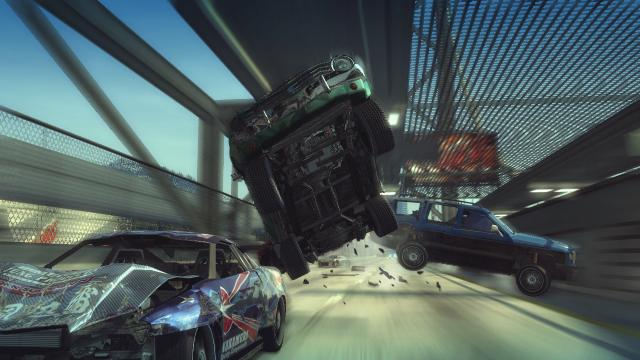
\includegraphics[height=0.3\textheight]{game} }
          % TODO честная полупрозрачность
          \only<2>{ 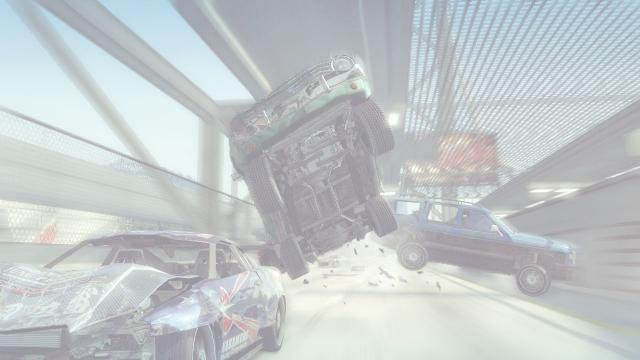
\includegraphics[height=0.3\textheight]{game-phantom} }

          Спецэффекты в кино

          \only<1>{ 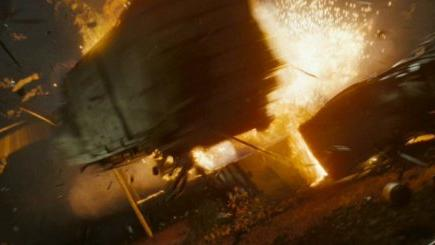
\includegraphics[height=0.3\textheight]{movie} }
          % TODO честная полупрозрачность
          \only<2>{ 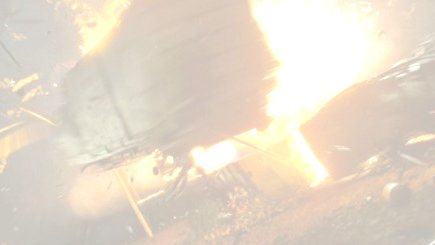
\includegraphics[height=0.3\textheight]{movie-phantom} }
        \end{center}
      \end{column}
      \begin{column}{0.5\textwidth}<-2>
        \begin{center}
          Обучающие тренажёры

          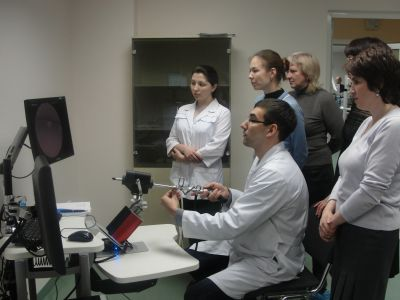
\includegraphics[height=0.3\textheight]{trainer}

          Системы авт. проектирования

          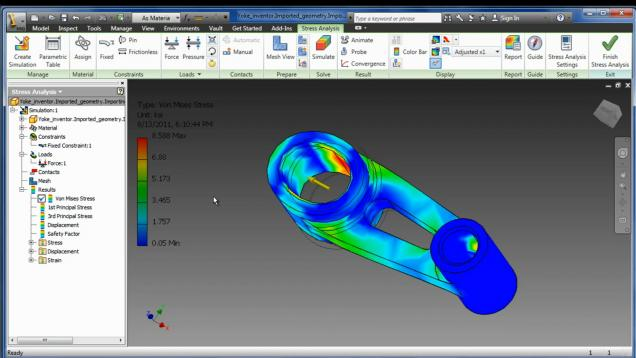
\includegraphics[height=0.3\textheight]{cad}
        \end{center}
      \end{column}
    \end{columns}
  \end{frame}
  \begin{frame}{Моделирование в реальном времени}
    В приложениях, связанных с визуализацией:
    % TODO круговые диаграммки
    \begin{enumerate}
      \item Мягкое реальное время.
      \item Комфорт пользователя: FPS $\ge 30$.
      \item За $\Delta t \le 33$~мс --- \emph{все} расчёты очередного кадра.
      \item На моделирование деформаций отводится $\Delta t' \approx 3..10$~мс.
    \end{enumerate}
  \end{frame}

  \begin{frame}{Актуальность}
    Разработка такой системы актуальна:
    \begin{itemize}
      \item применение систем виртуальной реальности в~обучении;
        % NB: сказать про перспективы 3D-печати тканей,органов...
      \item потребность в САПР протезов, имплантантов;
      \item отсутствие отечественных аналогов.
    \end{itemize}

    \vspace{1cm}
    
    Недостатки зарубежных аналогов (ANSYS, DEFORM-3D):
    \begin{itemize}
      \item не для моделированию биологических объектов;
      \item нельзя применить к расчётам в реальном времени;
      \item высокая цена.
    \end{itemize}
  \end{frame}

  \begin{frame}{Цель}
    \begin{block}{Цель проекта}
      Разработка \alert{системы моделирования} пластических деформаций биологических объектов
      \alert{в~реальном времени}, которая может быть использована как отдельно, так и в качестве
      \alert{модуля} для встраивания в стороннее приложение.
    \end{block}

    \vspace{0.5cm}

    Задачи:
    \begin{enumerate}
      \item Разработка \textcolor{ForestGreen}{алгоритма} моделирования
      \item Реализация \textcolor{ForestGreen}{его} в виде \textcolor{RoyalPurple}{программной библиотеки}
      \item Разработка на \textcolor{RoyalPurple}{её} основе \textcolor{NavyBlue}{интерактивного приложения}
    \end{enumerate}
  \end{frame}

  \section{Содержание проекта}
  \subsection{Содержание проекта}
  \begin{frame}{Научная новизна}
    \begin{enumerate}
      \item Собственные наработки по моделированию деформаций:
        \begin{itemize}
          \item объединение физических методов с геометрическими;
          \item разбиение 3D-модели на кластеры, подбор оптимального линейного преобразования для
            каждого;
          \item применение графического процессора.
        \end{itemize}
      \item Гибкий программный интерфейс (API).
      \item Адаптация алгоритма к физическим свойствам биологических объектов.
    \end{enumerate}
  \end{frame}

  \begin{frame}{Имеющийся задел}
    \begin{center}
      Работающий прототип

      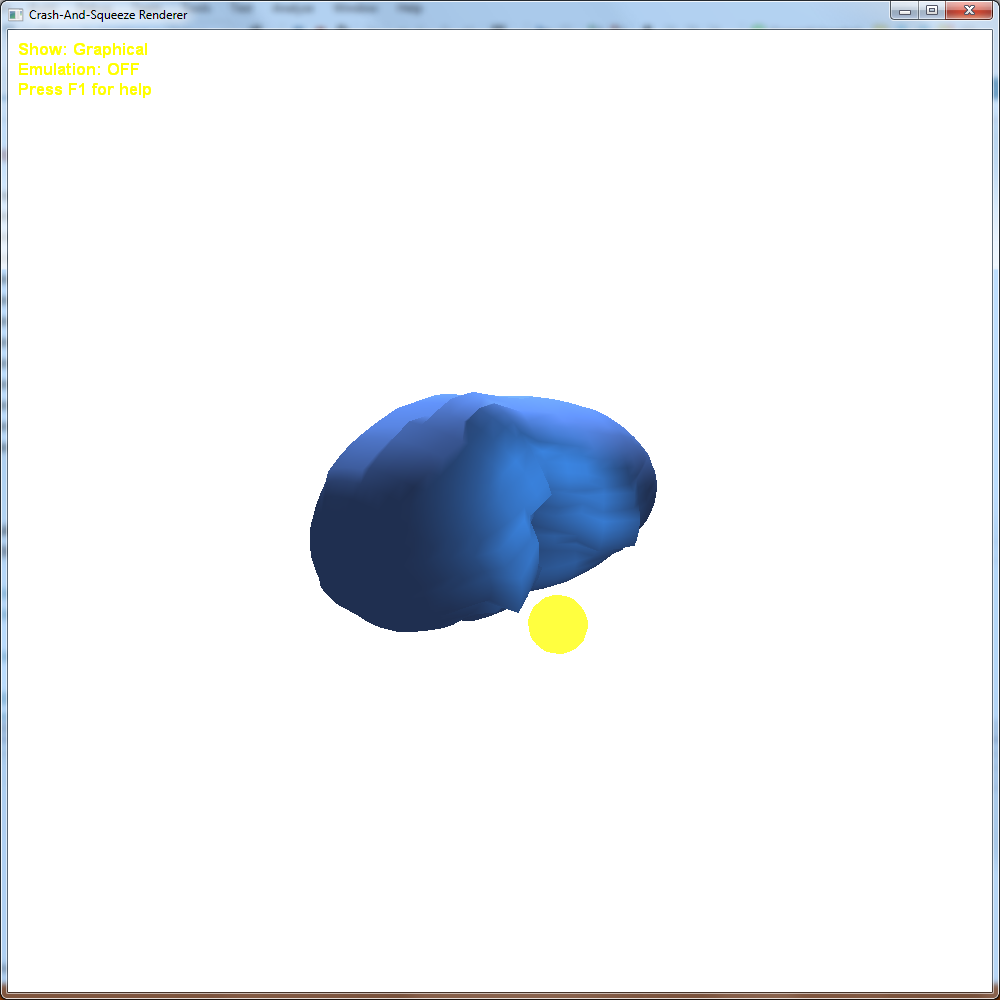
\includegraphics[height=0.7\textheight]{prototype}
    \end{center}
  \end{frame}

  \begin{frame}{Потенциальные заказчики}

  \end{frame}

  \begin{frame}{Коммерциализация}

  \end{frame}

  \section{План проекта}
  \subsection{План проекта}
  \begin{frame}{Календарный план}

  \end{frame}

  \begin{frame}{Перспективы и риски}

  \end{frame}

  \begin{frame}{Ожидаемый результат}

  \end{frame}


  % Заканчиваем последний section, чтобы заключение, "спасибо" и запасные слайды к нему не
  % относились и не отображались в навигации сверху
  \section{}

  \begin{frame}[plain]
    \begin{center}
      { \Huge Спасибо за внимание! }

      \vspace{1cm}

      Иван Новиков\\
      \url{http://about.me/moonlighter}\\
      \href{mailto:nia.afti@gmail.com}{\nolinkurl{nia.afti@gmail.com} }
      
    \end{center}
  \end{frame}

\end{document}

